\documentclass[UTF8]{ctexart}
\usepackage{amsmath}
\usepackage{amssymb}
\usepackage{booktabs}
\usepackage{background}
\usepackage{caption,subcaption}
\usepackage{diagbox}
\usepackage{enumitem}
\usepackage{float}
\usepackage{fontspec}
%\usepackage{fourier}
\usepackage{geometry}
\usepackage{makecell}
\usepackage{tikz}
\usetikzlibrary{arrows.meta}
\usepackage{xcolor}

\geometry{a5paper, top=0.1cm, left=1cm, right=1cm, bottom=0.3cm, footskip=0.1cm}
\setCJKmainfont[BoldFont={汉仪文黑-85W},ItalicFont={方正苏新诗柳楷简体}]{汉仪文黑-55W}
\setfontfamily\Issue{Century Schoolbook}
\setfontfamily\Genshin{Genshin Teyvat Lingua Franca}
\newCJKfontfamily\TitleFont{思源宋体 CN Heavy}
\newfontfamily\timesnewroman{Times New Roman}
\captionsetup{font=small, labelfont=bf}
\setlist[itemize]{itemsep=0pt, parsep=0pt}
%\reversemarginpar

%\CTEXsetup[format = {\centering\bfseries\large}, beforeskip = 3pt, afterskip = 3pt]{section}
\CTEXsetup[format = {\color{cyan!50!black}\bfseries\large}]{subsection}

\colorlet{darkcyan}{cyan!50!black}
\newcommand\Black[1]{\textcolor[gray]{0.3}{#1}}
\newcommand\Brown[1]{\textcolor[HTML]{998A4E}{#1}}
\newcommand\Emph[1]{\colorbox{green!10}{\textcolor{green!30!black}{#1}}}
\newcommand\Notes[1]{\textcolor{yellow!50!black}{\small #1}}
\newcommand\Example[1]{\textcolor{cyan!70!black}{\small #1}}


\newcommand\status[4]{\draw (#1 - 1,#2) circle (1) node{#3}; \draw (#1 + 1, #2) circle (1) node{#4};}
\renewcommand\d{\mathrm{d}}
\newcommand\Cov{\mathrm{Cov}}

\newcommand\IssueNumber{23}
\newcommand\Date{2024-4-12}
%\newcommand\Contributer{@金光日}
\newcommand\Subject{数字逻辑}
%\newcommand\Source{2021数 I 考研第 16 题}


\begin{document}
\backgroundsetup{contents=
\includegraphics{上半示例.png}, center, scale=1, angle=0, opacity=1}
\BgThispage
\begin{center}
%{\scriptsize\Issue \textcolor[HTML]{C8BA83}{\Genshin WEEKLY TIPS}}
\phantom{...}

{\Large\textcolor{brown!40!white}{\makebox[10cm][s]{\Genshin WEEKLY KNOWLEDGE TIPS}}}

\vspace{-2em}

{\Huge\bfseries\TitleFont \Black{知\ 识\ 小\ 料}}


\vspace{-0.1cm}
{\footnotesize \Brown{「电计 2203 班」周常规知识整理共享}}
\end{center}

\vspace{-0.5cm}


\begin{figure}[H]
\hspace{1cm}
\begin{minipage}[t]{0.3\textwidth}
\centering
    \Brown{\Genshin ISSUE}

    \vspace{-0.6cm}
    \Huge \Issue\slshape\bfseries\Black{\IssueNumber}
\end{minipage}
\hfill
\begin{minipage}[t]{0.35\textwidth}
\small
\centering
    \Brown{日期:\Date} \\
%\vspace{-0.1cm}
%    \Brown{贡献者:\Contributer} \\
\vspace{-0.1cm}
    \Brown{学科:\Subject} \\
\end{minipage}
\hspace{0.8cm}
\end{figure}

{\color{cyan!50!black} 使用两个计数器 74290,连接成模 12(8421BCD 码)电路,假设初始值从 0 开始,并按照图例指示,画出状态图。

\begin{figure}[htb]
  \centering
  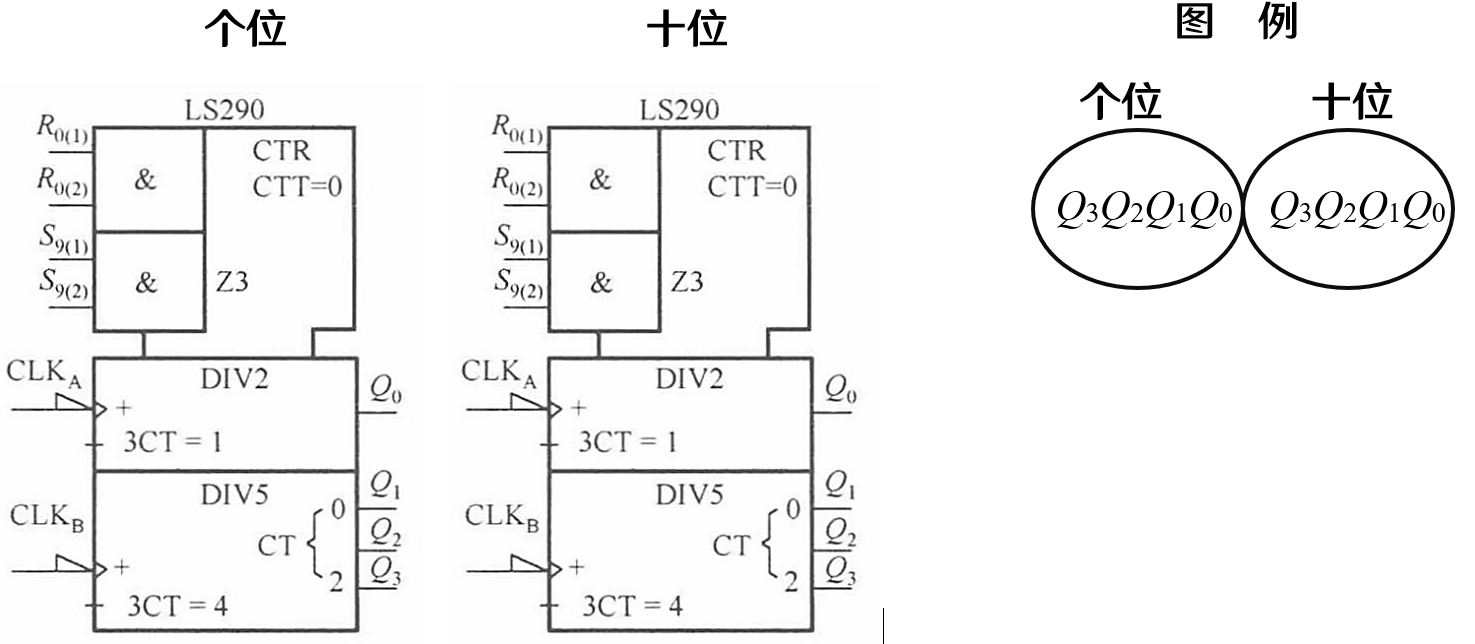
\includegraphics[width=12cm]{题目.png}
\end{figure}
}

74290 是二·五·十进制异步加法计数器,级联时考虑这些:
\begin{itemize}
    \item 单片模 10,因此将各自的 $Q_0$ 与 $\mathrm{CLK_B}$ 接起来。
    \item 总共 12 个状态从 0000,0000 到 0001,0001(十位,个位),即 $0\sim 11$,当达到 0001,0010 时触发异步复位。
    \item 将个位片的 $Q_3$ 和十位片的 $\mathrm{CLK_A}$ 接起来,以实现进位。\textcolor{cyan}{(因为当个位片从 $1001\to 0000$ 时,$Q_3$ 恰好是下降沿,可作为十位片时钟 A 触发的信号)}
\end{itemize}

\vspace{-1cm}
\begin{table}[htb]
  \centering
  \begin{tabular}{cccccccccc}
  \toprule
  十进制 & $Q_3'$ & $Q_2'$ & $Q_1'$ & $Q_0'$ & $Q_3$ & $Q_2$ & $Q_1$ & $Q_0$ \\
  \midrule
  0& 0&0&0&0&0&0&0&0 \\
  1& 0&0&0&0&0&0&0&1 \\
  $\vdots$ & $\vdots$ & $\vdots$ & $\vdots$ & $\vdots$ & $\vdots$ & $\vdots$ & $\vdots$  \\
  9& 0&0&0&0&1&0&0&1 \\
  10& 0&0&0&1&0&0&0&0 \\
  11& 0&0&0&1&0&0&0&1 \\
  12& 0&0&0&1&0&0&1&0 & 暂态归零 \\
  \bottomrule
  \end{tabular}
\end{table}

\newpage
\backgroundsetup{contents=
\includegraphics{下半示例.png}, center, scale=1, angle=0, opacity=1}
\BgThispage

上表中,$Q_3'Q_2'Q_1'Q_0'$ 为十位片输出,$Q_3Q_2Q_1Q_0$ 为个位片输出。

因此能够得到连接方式和状态图,如下图所示。
\begin{figure}[htb]
  \centering
  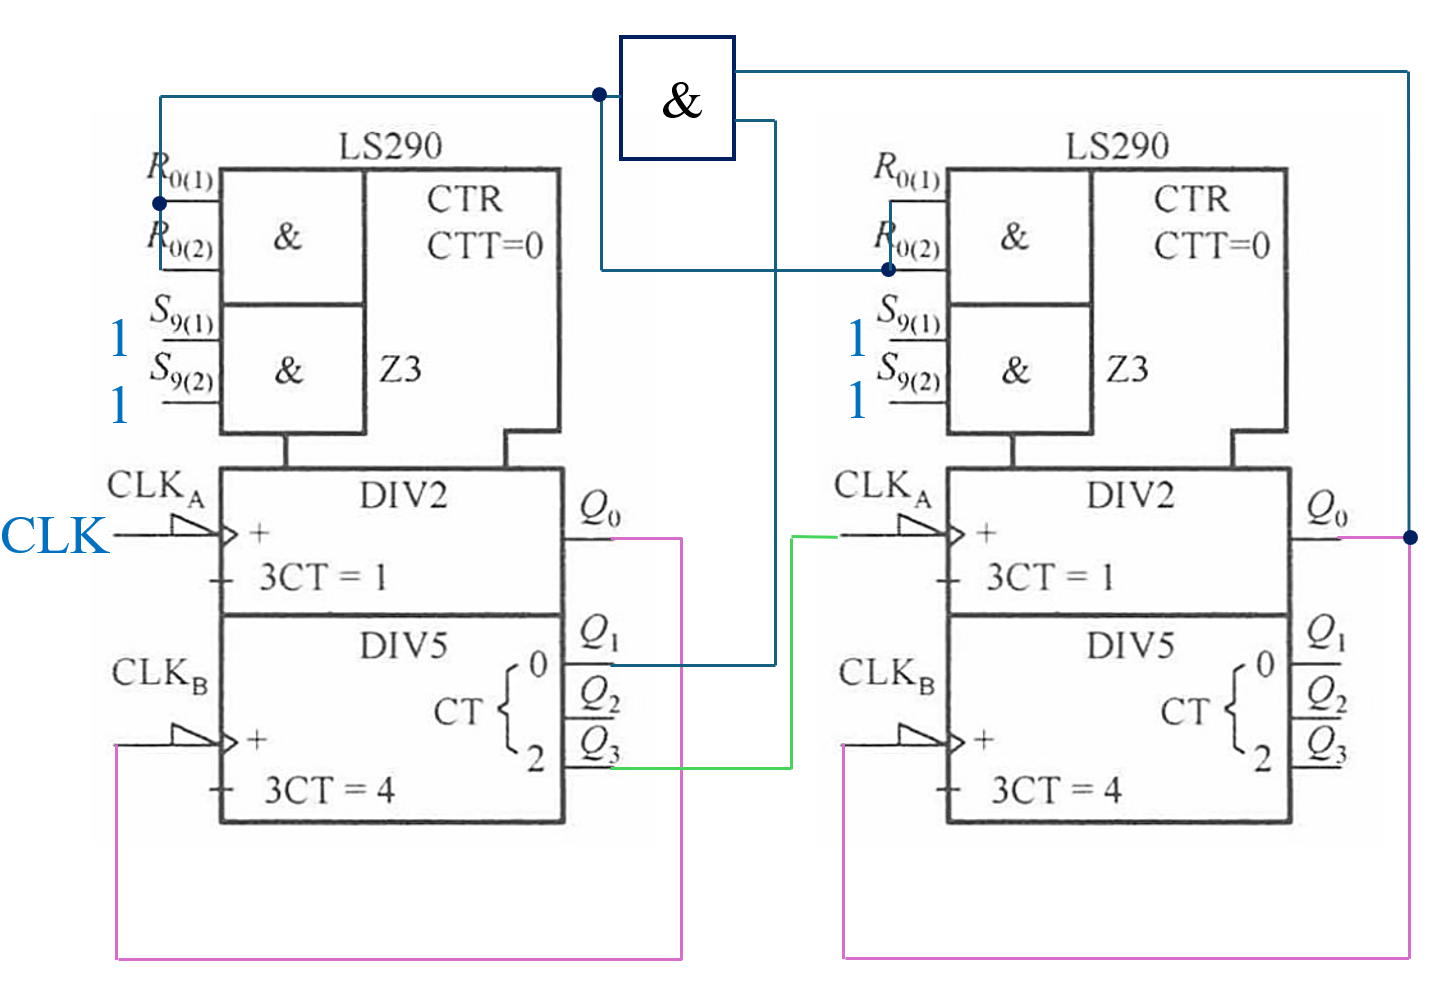
\includegraphics[width=10cm]{答案.png}
\end{figure}

\begin{figure}[htb]
  \centering
  \begin{tikzpicture}[>=Stealth, scale=0.5]
    \status{0}{6}{0000}{0000}
    \status{5}{6}{0001}{0000}
    \status{10}{6}{0010}{0000}
    \status{15}{6}{0011}{0000}
    \status{15}{3}{0100}{0000}
    \status{15}{0}{0101}{0000}
    \status{15}{-3}{0110}{0000}
    \status{10}{-3}{0111}{0000}
    \status{5}{-3}{1000}{0000}
    \status{0}{-3}{1001}{0000}
    \status{0}{0}{0000}{0001}
    \status{0}{3}{0001}{0001}
    \draw[->] (2,6) -- (3,6);
    \draw[->] (7,6) -- (8,6);
    \draw[->] (12,6) -- (13,6);
    \draw[->] (15,5) -- (15,4);
    \draw[->] (15,2) -- (15,1);
    \draw[->] (15,-1) -- (15,-2);
    \draw[->] (13,-3) -- (12,-3);
    \draw[->] (8,-3) -- (7,-3);
    \draw[->] (3,-3) -- (2,-3);
    \draw[->] (0,-2) -- (0,-1);
    \draw[->] (0,1) -- (0,2);
    \draw[dashed] (7,3) circle (1) node{0010}; 
    \draw[dashed] (9, 3) circle (1) node{0001};
    \draw[dashed,->] (2,3) -- (6,3) node[midway, font=\footnotesize] {暂态};
    \draw[dashed,->] (6.106,3.447) -- (1.894,5.553) node[midway, sloped, font=\footnotesize] {异步置零};
  \end{tikzpicture}
\end{figure}

\vspace{1em}
{\color{cyan!80!black} 【结论】见解析

【点评】本题考察了模二·五·十计数器 74290 的级联用法,考察了对计数、异步置零、进位等功能的理解。画出状态表,根据状态表设计电路,并顺势画出状态图,即可完成本题。
}

\end{document}